\chapter{Взаимодействие симуляции с~внешним миром}\label{chapter13}

\dictum[Дмитрий Гайдук. Про олдовых людей]{Мимо люди разные ходят, но никто внимания не обращает: эка невидаль, в~самом деле, два олдовых человека реальность проткнуть пытаются.}

\section[Необходимость взаимодействия]{Необходимость взаимодействия симуляции и реальности}

Как и большинство прикладных программ, симуляторы не создаются по мотивам философской концепции «вещи в себе», а имеют средства взаимодействия с человеком. Пользователю необходимо как вводить некоторые данные в систему, так и получать её отклик, ради которого она и создавалась. Выделим два класса для таких активностей.

\begin{enumerate*}
\item \textit{Взаимодействие с моделью, повторяющее действия, осуществляемые с её физическим прототипом.} Если у реального компьютера есть клавиатура и оператор может нажимать её клавиши, нечто аналогичное должно быть у симулируемой модели. Если в конфигурации присутствует монитор или иное средство для вывода информации, оно в той или иной форме должно быть и в модели. 

\begin{figure}[htp]
    \centering
    % \includegraphics[width=0.8\textwidth]{./isolate-crop.pdf}
\begin{tikzpicture}[>=latex, font=\small, node distance=0.3cm, inner sep=0pt]
    
    \node (tower) {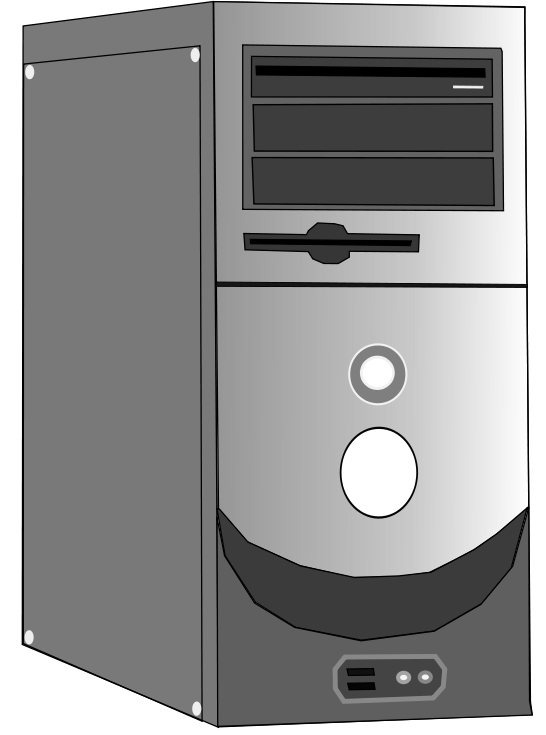
\includegraphics[height=1.5cm]{./tower.png}};
    \node[above=of tower] (monitor1) {
\includegraphics[height=1.2cm]{./monitor1.png}};
    \node[right =0.2cm of monitor1] (kb1) {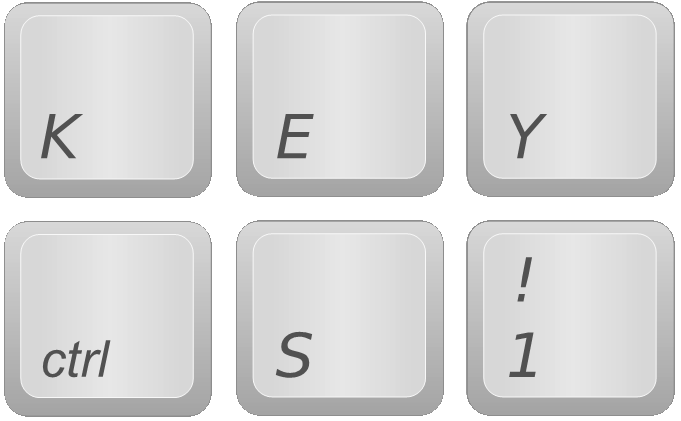
\includegraphics[height=.8cm]{./kb1.png}};
    
    % Inner border
    \node[draw, inner sep=0.2cm, fit=(tower) (monitor1) (kb1)] (virt) {};
    
    \node[right =2.cm of tower] (folder) {
\includegraphics[height=1.cm]{./folder.png}};
    \node[right =0.2cm of folder] (hdd) {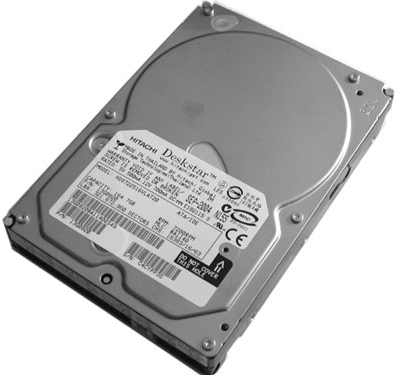
\includegraphics[height=1.cm]{./device3.png}};
    
    \node[right=0.7cm of hdd] (stub) {};
    
    % The outer border
    \node[draw, inner sep=0.35cm, fit= (virt) (tower) (monitor1) (kb1)  (hdd) (stub)]  (real) {};
    
    \node[right =0.2cm of hdd] (nic) {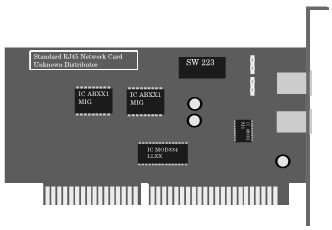
\includegraphics[height=1.cm]{./nic.png}};
    \node[right =of kb1, yshift=1cm] (kb2) {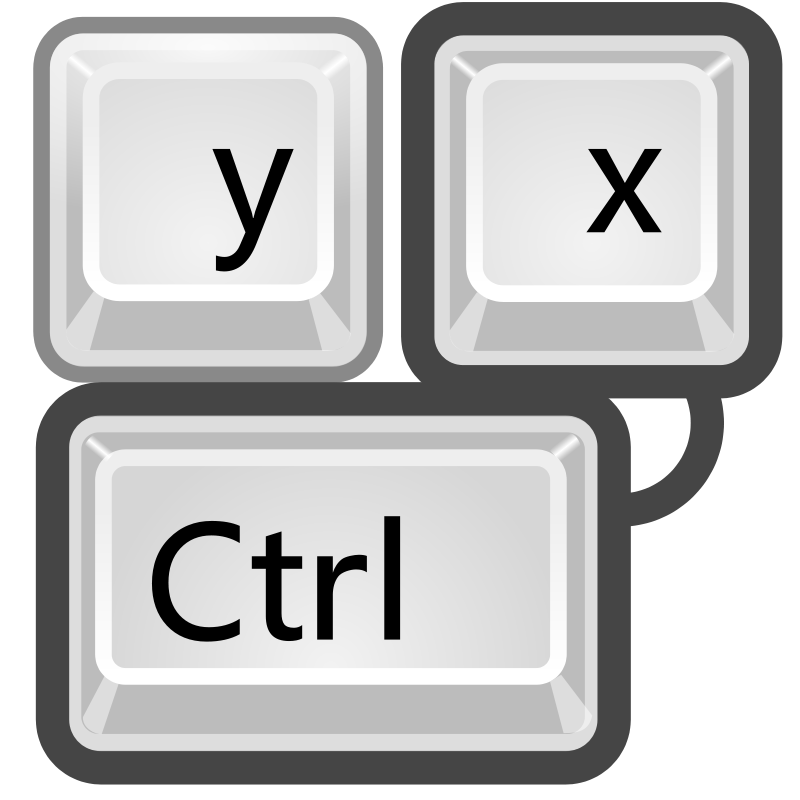
\includegraphics[height=1.5cm]{./kb2.png}};
    \node[right =of kb2] (monitor2) {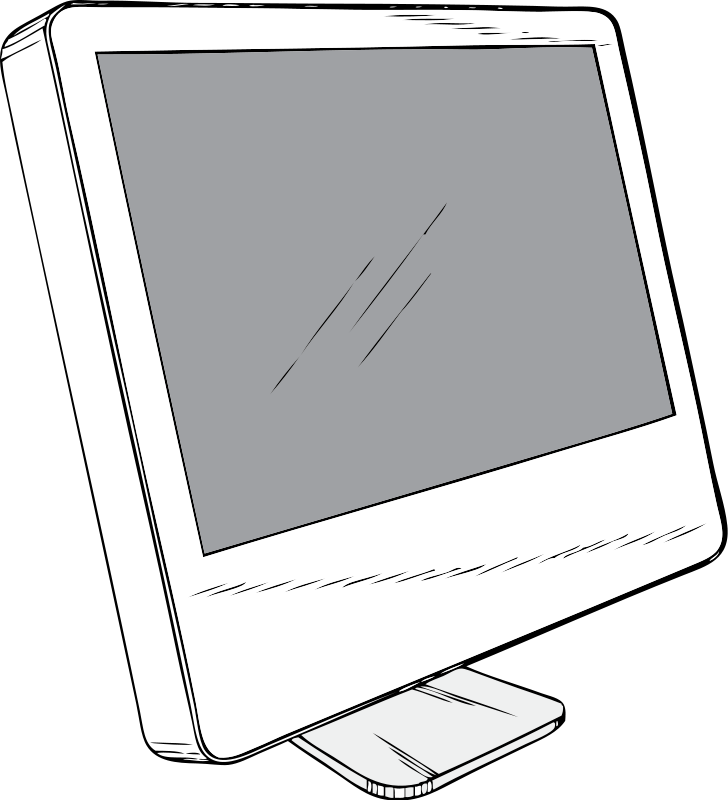
\includegraphics[height=1.5cm]{./monitor2.png}};   
    
    \node[fill=white, font=\scriptsize] at (virt.south) {Граница ВМ};
    
    \node[fill=white, font=\scriptsize] at (real.south) {Граница реальной системы};
\end{tikzpicture}
    \caption{Изоляция симулируемой системы от внешней среды}
    \label{fig:isolate}
\end{figure}

Симулируемое окружение вступает во взаимодействие с настоящим миром, находящимся вне модели, со всеми вытекающими из этого обстоятельствами, например невозможностью гарантировать повторяемость симуляций: даже если человек нажимает одни и те же клавиши в различных запусках модели, длительность и паузы между ними всегда будут различными.

Отметим, что полная аналогичность пользовательского интерфейса необязательна --- так, ввод с клавиатуры для модели на самом деле может идти из заранее записанного файла, расположенного на хозяйской файловой системе, а вывод видеокарты --- сохраняться в сетевой поток, транслируемый на удалённый сервер.

\item \textit{Инспектирование состояния модели и вмешательство в её работу, неосуществимые на реальной аппаратуре.} Сюда входит чтение содержимого регистров, памяти, их изменение «вручную», остановка симулируемого времени и т.п. Такие действия чаще всего не имеют соответствия в сценариях работы аппаратуры в реальном мире.
\end{enumerate*}

\section{Паравиртуализационные расширения}

Согласно принципу полной изоляции виртуализированного окружения находящаяся в нём программа не должна иметь возможностей отличить ситуацию, когда она выполняется на реальной аппаратуре, от работы внутри виртуального окружения. Это условие очень важно, так как позволяет использовать одно и то же программное обеспечение без необходимости модификаций и применять результаты, полученные на модели (доказательства корректности, предсказания производительности, энергопотребления и т.п.), к реальности.

Однако часто оказывается выгодным «пробить» изоляцию для увеличения производительности симуляции, повышения удобства пользования или получения новых сценариев взаимодействия окружений. При этом гостевое приложение или ОС модифицируются таким образом, чтобы задействовать некоторую функциональность аппаратуры, присутствующую только внутри модели, но не на реальных системах. Этот приём имеет общее название \textbf{паравиртуализация}.

\subsection{Волшебные инструкции}

Для того чтобы иметь возможность совершать некоторые действия по достижении приложением некоторого этапа своей работы, можно использовать \textit{точки остановки симуляции} (\abbr breakpoints) по значению регистра-счётчика текущей инструкции. Иногда удобнее реагировать на исполнение некоторой специально выбранной инструкции вне зависимости от её адреса. В таком случае инструкция получает название «волшебной», т.к. с ней связаны необычные эффекты. С помощью такой инструкции мы можем помечать в приложении интересующие места, при этом на неё налагаются следующие ограничения.

\begin{itemize*}
\item    Инструкция не должна использоваться самим приложением, иначе мы будем получать ложные срабатывания и будем вынуждены как-то фильтровать их.
\item    Желательно, чтобы она несла минимальную семантическую нагрузку, что позволило бы использовать её во многих сценариях. Так, желательно, чтобы инструкция не была неопределённой на реальной аппаратуре, иначе приложение с ней не будет корректным вне симулятора. 
\item В идеале она должна сохранять неизменным содержимое памяти, работать во всех режимах процессора, предсказуемо менять счётчик инструкций, т.е. не быть инструкцией перехода. 
\end{itemize*}

Второму условию наилучшим образом отвечают варианты инструкции NOP --- no operation. В самом деле, подобная инструкция изменяет архитектурное состояние минимальным образом (т.к. на её исполнение всё-таки тратится время). Однако компиляторы часто используют NOP для своих целей выравнивания кода и т.п., что не соответствует первому условию. Исключением является архитектура IA-32, где имеются две инструкции NOP --- классическая однобайтовая (\texttt{0x90}) и  расширенная (\texttt{0x0F 0x1F /0})~\cite{intelmanual2a}; последняя может иметь длину от трёх до девяти байт и один операнд. Она является хорошим кандидатом для того, чтобы стать «волшебной» внутри симуляции.

Другой альтернативой являются недокументированные инструкции, которые не встречаются в приложениях. Однако их неопределённая функциональность на реальной аппаратуре ограничивает удобство использования.

Третьим вариантом можно считать инструкции с необычными аргументами, префиксами и другими особенностями, не встречающиеся в обычном коде. Например, для архитектуры IA-32 это может быть \texttt{CPUID} с операндами вне допустимого диапазона, инструкции с префиксами, не влияющими на её исполнение и т.п.

\begin{figure}[htp]
    \centering
    % \includegraphics[width=0.6\textwidth]{./magic-inst-crop.pdf}
\begin{tikzpicture}[>=latex, font=\small]
    \node (tower) {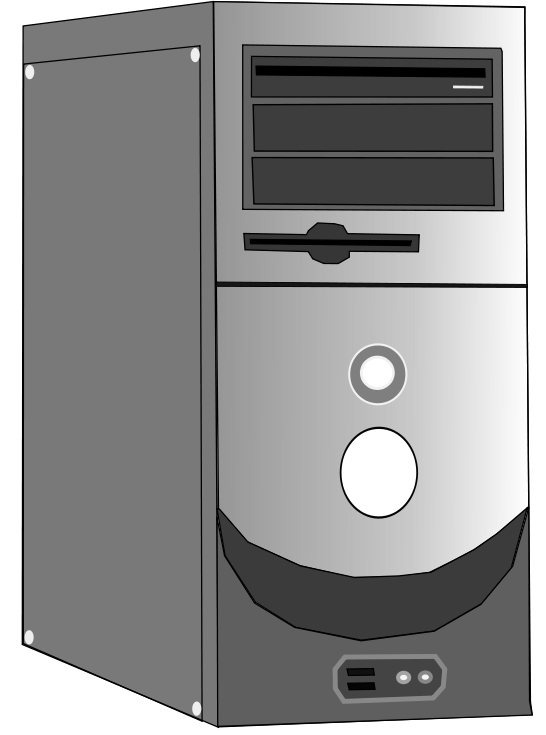
\includegraphics[height=1.5cm]{./tower.png}};
    \node[right =0.25cm of tower] (folder1) {
\includegraphics[height=1.cm]{./folder.png}};
    \node[right=0.5cm of folder1] (stub) {};
    \node[draw, fit=(tower) (folder1) (stub), inner sep=2pt] (virt) {};
    
    \node[right =0.1cm of folder1, double arrow, draw, fill=white] (arrow) {1 байт};
    \node[right =0.1cm of arrow] (folder2) {
\includegraphics[height=1.cm]{./folder.png}};
    \node[draw, fit=(tower) (folder1) (folder2), inner sep=0.5cm] (real) {};
    
    \node[fill=white, font=\scriptsize, inner sep=1pt] at (virt.south) {Граница ВМ};
    \node[fill=white, font=\scriptsize, inner sep=1pt] at (real.south) {Граница реальной системы};
\end{tikzpicture}    
    \caption{Передача файлов с помощью магических инструкций}
    \label{fig:magic-inst}
\end{figure}

\subsection{Паравиртуальные устройства}

Сценарий использования «волшебной» инструкции, описанный ранее, передаёт лишь один бит информации между гостем и хозяином --- это сам факт присутствия. Часто возникает необходимость передать большие объёмы информации. Несколько байт ещё могут вместиться как операнды инструкции или в регистрах процессора. Для передачи большего объёма данных за один раз необходимо иметь больший буфер для данных. Самым очевидным представляется выделить для этого часть физического адресного пространства гостя. Чтобы чтения и записи этого диапазона обрабатывались симулятором, с ним ассоциируется псевдоустройство; запись в ассоциированную с ним память вызывает приостановку симуляции и обработку новых данных. О способе использования этого механизма рассказывается в следующей секции.

\subsection[Ускорение ввода-вывода]{Ускорение ввода-вывода через периферийные устройства}

Виртуализация выступает как дополнительная «обёртка» между виртуальными и реальными устройствами ввода-вывода (установленными в PCI, PCI-Express слоты расширений, подключенными к IDE и SATA шинам дисками и т.п.), что приводит к необходимости двойной (иногда тройной) передаче данных --- один раз внутри модели, второй --- в реальной системе. Это приводит к копированию больших объёмов данных из одной области памяти в другую без какой-либо обработки и сильно ограничивает скорость работы высокоскоростных периферийных устройств.

Для ускорения необходимо избавиться от прослойки симуляции для определённых устройств. Реализуется это модификацией гостевой операционной системы --- в неё включаются драйвера паравиртуальных устройств, способных напрямую инструктировать виртуальную машину о необходимости передачи данных.

Изменённое ядро является недостатком этого подхода и существенно ограничивает его применимость для систем, коды/интерфейсы ядра которых закрыты.

\subsection{Проброс устройства}

Иногда представляется возможным перенаправлять все запросы на доступ к некоторому устройству прямо из гостя, без обработки команд симулятором. Это требует вмешательства уже в хозяйскую ОС, так как обычно она ограничивает  прямой доступ к аппаратуре со стороны пользовательских приложений.

В случае паравиртуализации периферийное устройство может быть разделено между хозяином и несколькими гостями. При \textbf{пробросе} чаще всего оно полностью отдано одному из них. Пример эксклюзивного использования хозяйских устройств --- проброс USB-устройств в Oracle Virtualbox; при этом оно пропадает в хозяйской системе до тех пор, пока подключено к виртуальной машине.

В современных материнских платах появилась аппаратная поддержка виртуализации периферийных устройств, что избавляет виртуальные машины от ещё одного уровня косвенности --- он переносится в «железо». Что интересно, уровень позволяет также эффективно использовать одно устройство в нескольких независимых изолированных окружениях. Например, сетевая карта при этом будет иметь несколько независимых MAC-адресов, что зачастую избавляет от необходимости использования паравиртуализации. Примеры таких технологий --- Intel VTd и AMD IOMMU.

\subsection{Дополнительные каналы передачи данных}

Описанные выше техники в общем случае позволяют внести в симулируемое окружение дополнительные способы обмена данными между хозяином и гостем. При этом паравиртуализация может проявляться на разных уровнях программного стека гостевой ОС, а не только на уровне драйверов устройств. Например, <<волшебные инструкции>> могут быть использованы для реализации утилиты копирования  отдельных файлов (в общем случае --- потока байт) между гостем и хозяином. Если требуется более тесная интеграция, то может быть использован драйвер файловой системы для монтирования директории машины хозяина внутри гостя, при этом все изменения, сделанные внутри гостя, становятся видны снаружи в хозяине. Такая функциональность существует во многих популярных виртуальных машинах, например в виде файловых систем \texttt{hostfs} в составе Simics или \texttt{vboxsf} из состава гостевых дополнений Virtualbox.

\section[Интерактивные устройства]{Интерактивные устройства для~взаимодействия с пользователем}

Простейшее средство для общения пользователя с системой может быть представлено двумя односторонними потоками символов. Базовое устройство, предоставляющее такой функционал, --- это последовательный порт RS-232. Несмотря на приличный возраст стандарта и невысокую скорость передачи данных (до 115,2 кбит/c), он до сих пор является популярным интерфейсом для многих приложений, поддерживается практически всеми существующими операционными системами и доступен на самых ранних этапах загрузки ЭВМ. Часто именно этот вид периферийного устройства реализуется в новом симуляторе в первую очередь. 

Ввиду простоты используемой абстракции передачи данных модель последовательного порта со стороны реального мира может быть использована множеством способов. Например, возможно подключение к эмулятору терминала и использование модели для интерактивного взаимодействия с пользователем. Выходящий поток  будет записываться в файл, а ввод-вывод --- перенаправлен в сетевой сокет, именованный канал Unix/Windows, символьное  устройство или виртуальный параллельный порт или даже подключен к реальному порту хозяйской системы.

Более сложными с точки зрения моделирования устройствами ввода являются клавиатура и мышь. Существуют варианты их подключения к материнской плате через различные интерфейсы: последовательный порт, PS/2, USB\dots\ Клавиатура должна моделировать события нажатия и отпускания, а также допускать возможность одновременного нажатия нескольких клавиш. Способы подключения к реальности, как и в случае последовательного интерфейса, могут быть разнообразными.

Наиболее популярным устройством вывода графической информации является монитор. Его моделирование подразумевает создание сложного комплекса моделей: от PCI (Express) или AGP слотов на материнской плате до видеокарты, далее через цифровую начинку монитора к его дисплею. Серьёзная задача состоит в обеспечении достаточной скорости прорисовки изображения, формируемого гостем, особенно если это трёхмерные сцены или интенсивная двухмерная графика (видео). В таких сценариях использования «программная» эмуляция только средствами центрального процессора хозяина, как правило, неспособна обеспечить комфортную для пользователя частоту обновления экрана. Решение состоит в задействовании аппаратных ресурсов хозяйской машины, осуществляемое либо через паравиртуализацию, либо пробросом PCI устройства в гостевую систему.

\section{Диски}

Под дисками мы будем подразумевать устройства хранения данных на жёстких магнитных дисках (стандарты SATA, IDE, FireWire, SCSI), твердотельных накопителях (USB-флешки, SSD), а также оптические диски (CD, DVD, Blu-ray) и теряющие актуальность гибкие диски (\abbr floppy disks).

С моделированием дисковой подсистемы связано несколько специфичных вопросов.

\begin{itemize*}
\item Обеспечение высокой скорости симуляции. Объём передаваемых данных для ряда приложений может быть большим, как и связанное с этим замедление модели.

\item Обеспечение непосредственного хранения массивов данных. Ёмкость моделируемых дисков может достигать десятков терабайт.
\item Постоянство хранилища модели. В отличие от ОЗУ и регистров устройств, жёсткие диски не теряют данные при выключении или перезагрузке компьютера. Однако сохранение состояния между запусками симуляции нарушает принцип её воспроизводимости и повторяемости.
\end{itemize*}

\subsection{Скорость}

В общем случае замедление связано с необходимостью многократного копирования данных между симуляцией и реальной системой хранения. Как было описано раньше, сценарии решения этой проблемы заключаются в паравиртуализации или в пробросе устройства внутрь симуляции.

\subsection{Форматы хранения}

Поскольку диск представляет собой устройство с произвольным доступом, естественная форма хранения его данных --- это файл в хозяйской системе, блоки содержимого которого соответствуют данным гостевого диска.

В простейшем случае файл должен содержать просто копию байт-в-байт всего содержимого реального диска, это т.н. «сырой» (\abbr raw) образ диска (рис.~\ref{fig:raw}). При этом все сектора гостевого диска расположены последовательно в том же порядке, который они имели бы  в реальности. Преимущество такого способа хранения --- его простота и универсальность. Создание образа диска из существующего физического элементарно\footnote{Например, с помощью Unix-утилиты \texttt{dd}.}. Практически все существующие симуляторы поддерживают образы в <<сыром>> формате. Основной его недостаток --- нерациональность использования ресурсов хозяина. Например, симуляция установки ОС может занять 1 Гбайт места на образе диска в 100 Гбайт; результирующий образ диска будет занимать 100 Гбайт, при этом 99\% его будут потеряны для хозяйской системы впустую.

\begin{figure}[htb]
    \centering
    % \includegraphics[width=0.8\textwidth]{./raw-format-crop.pdf}
\begin{tikzpicture}[>=latex, font=\small]
    \path (0,0.5) coordinate (a1);
    \draw (0,0) rectangle (7.5,1);
    \node[left = 0.25cm of a1] (host-disk) {Хозяйский диск};
    
    \draw (3,-2) rectangle (6,-1);
    \node[below = 1.5cm of host-disk] {Гостевой диск};
    
    \draw[fill=black!5] (3,0) rectangle (6,1);
    \draw[dotted] (3,-1) -- (3,0);
    \draw[dotted] (6,-1) -- (6,0);
    
    \path[fill=black!20] (4,0) rectangle (4.5,1);
    \path[fill=black!20] (5,0) rectangle (5.5,1);
    
    \path[fill=black!20] (4,-2) rectangle (4.5,-1);
    \path[fill=black!20] (5,-2) rectangle (5.5,-1);
    
    \draw[<->] (4.25,-1) -- (4.25,0);
    \draw[<->] (5.25,-1) -- (5.25,0);
    
    \path (4.5,-2) coordinate (a2);
    \node[below =0.25cm of a2, inner sep=1pt] (used) {Используемые области};
    
    \draw[dotted] (used) -- (4.25,-2);
    \draw[dotted] (used) -- (5.25,-2);
    
    \draw[decorate, decoration={brace, amplitude=3pt}, yshift=3pt] (3,1) -- (6,1) coordinate[midway] (a3);
    \node[above = 0.1cm of a3] {Образ диска};    
\end{tikzpicture}
    \caption[<<Сырой>> образ диска]{<<Сырой>> образ диска. Хранится каждый сектор, даже если он не задействоован внутри гостевой системы, что приводит к нерациональному расходованию места}
    \label{fig:raw}
\end{figure}

Многие симуляторы поддерживают более компактные способы хранения, в которых в файл записываются только изменённые секторы диска; заголовочная часть файла содержит список этих секторов и их местоположение (рис.~\ref{fig:compat}). Как правило, каждая программа имеет свой формат и иногда поддерживает другие или позволяет конвертировать их друг в друга. Примеры: Qcow2~\cite{qcow2} (Qemu), VDI (Oracle Virtualbox), VMDK~\cite{vmdk} (VMware ESX), VHD (Microsoft VirtualPC), HDD (Parallels Desktop), CRAFF (Wind River Simics).

\begin{figure}[htb]
    \centering
    % \includegraphics[width=0.8\textwidth]{./compat-crop.pdf}
\begin{tikzpicture}[>=latex, font=\small]
    \path (0,0.5) coordinate (a1);
    \draw (0,0) rectangle (7.5,1);
    \node[left = 0.25cm of a1] (host-disk) {Хозяйский диск};
    
    \draw (3,-2) rectangle (7,-1);
    \node[below = 1.5cm of host-disk] {Гостевой диск};
    
    % \draw[fill=black!5] (3,0) rectangle (6,1);
    % \draw[dotted] (3,-1) -- (3,0);
    % \draw[dotted] (6,-1) -- (6,0);
    
    \path[thick, fill=black!25] (1.2,0) rectangle (1.49,1);
    \path[fill=black!20] (1.51,0) rectangle (2.49,1);
    \path[fill=black!20] (2.51,0) rectangle (3.5,1);
    
    \path[fill=black!20] (4.,-2) rectangle (4.99,-1);
    \path[fill=black!20] (5.01,-2) rectangle (6,-1);
    
    \draw[<->] (4.25,-1) -- (2,0);
    \draw[<->] (5.25,-1) -- (3,0);
    
    \path (4.5,-2) coordinate (a2);
    \node[below =0.25cm of a2, inner sep=1pt] (used) {Используемые области};
    
    \draw[dotted] (used) -- (4.25,-2);
    \draw[dotted] (used) -- (5.25,-2);
    
    \draw[decorate, decoration={brace, amplitude=3pt}, yshift=3pt] (1.2,1) -- (3.5,1) coordinate[midway] (a3);
    \path (1.35,1) coordinate (a4);
    \node[above = 0.1cm of a3] {Образ диска};    
    \node[above = 0.5cm of a4, xshift=-2cm, inner sep=1pt] (header) {Заголовок};    
    \draw[dotted] (a4) -- (header);
    
\end{tikzpicture}
    \caption[Компактный формат образа диска]{Компактный формат образа диска. Хранятся только данные используемых секторов гостевого диска, а также служебная информация, описывающая их местоположение}
    \label{fig:compat}
\end{figure}

Некоторые форматы поддерживают прозрачное сжатие записанных данных, когда вместо обычной копии каждого гостевого сектора хранится его представление, полученное применением одного из известных алгоритмов сжатия без потерь, например Gzip, Bzip2 или LZMA~\cite{sayood2002lossless}.

Для образов оптических дисков, которые в большинстве  случаев являются носителями с данными только для чтения, используются сырые образы. Чаще всего они именуются ISO-образами по имени стандарта используемой на них файловой системы ISO 9660\footnote{Хотя это не единственный стандарт для оптических дисков; альтернативой является UDF (universal disk format), призванный обойти многие ограничения ISO 9660.}.

Из-за своего небольшого размера (меньше 3 Мбайт) образы гибких дисков хранятся в raw-формате.

\subsection{Сохранение состояния дисков}

Зачастую нежелательно модифицировать исходный файл образа диска: экспериментальное ПО/вирусы/ошибки пользователя внутри симулятора могут сделать его неработоспособным, или же желательно впоследствии запускать симуляцию из первоначального состояния.

Для таких целей в большинстве симуляторов существует опция: все изменённые секторы сохранять не в оригинальном, а в дополнительном \textbf{разностном} файле (также называемом \textbf{дельтой}). Для моделируемого приложения указанная схема абсолютно прозрачна --- внутри симуляции изменения видны там, где и должны быть. Однако после выключения симуляции допустимо отбросить дельту и использовать оригинальный образ. В случае появления желания зафиксировать внесённые в результате последней симуляционной сессии правки --- следует воспользоваться утилитами слияния оригинального образа и дельты.

Развивая эту идею, можно вообразить себе схему с несколькими дельтами, полученными на разных этапах симуляции (и даже <<дельты к дельтам>>), одновременно наложенными на диск. Таким образом, можно иметь множество снимков состояний дискового хранилища, суммарно занимающие места меньше, чем занимали бы отдельные полные копии.

\section{Сеть}

Современный Интернет был спроектирован так, чтобы обеспечивать обмен информацией между системами совершенно различной структуры, масштабов, используемых технологий. Взаимодействие симуляции и реальности через сеть является наиболее «естественным» подходом, поскольку у агентов имеются лишь самые общие предположения о свойствах друг друга.

Существует семь уровней абстракции данных OSI ISO~\cite{osi-iso-rus}. Ниже описана возможная классификация способов взаимодействия хозяина и гостя по их соответствию некоторым из этих уровней. Отметим, что такая классификация не является строгой и приводится для подчёркивания различий между ними.

\begin{itemize*}
\item    \textit{Физический уровень}. Для прозрачного использования гостевыми системами хозяйской сети необходимо иметь работающую модель сетевой карты (\abbr network interface card, NIC). Она может быть соединена с другими чисто программными моделями сетевых устройств (NIC, маршрутизаторами и т.д.) внутри симуляции или представлять собой проброшенную в симуляцию физическую NIC хозяйской системы.

\item    \textit{Канальный уровень}. Драйвер, именуемый TAP~\cite{tuntap}, обеспечивает модель сетевой карты и работает с кадрами Ethernet. Он устанавливается в хозяине. После этого хозяйская система может через новый интерфейс псевдо NIC взаимодейстовать с гостевой системой (при условии правильной настройки адресов и маршрутизации). Для того чтобы гость был представлен в том сегменте реальной сети, в котором находится хозяин, необходимо объединить в мост (\abbr bridge) одну из реальных и виртуальную карты. Очевидный недостаток --- хозяин теряет одно устройство NIC на каждой симуляции.

\item     \textit{Сетевой уровень}. TUN-драйвер обеспечивает более высокоуровневую модель и оперирует IP-пакетами, а не кадрами Ethernet. Такое соединение может использоваться для создания сетевого туннеля, например VPN. С точки зрения целей симуляции TUN не предоставляет существенных преимуществ над TAP.

\item    \textit{Транспортный уровень}. Для одностороннего доступа гостей к внешней сети, как правило, используется решение, в котором он размещается в отдельной подсети, а хозяин выступает как NAT-сервер. Все исходящие TCP-соединения выглядят как исходящие от хозяина. Недостаток данного подхода состоит в невозможности открыть соединение извне с симуляцией. Для обхождения этой проблемы используют переадресацию фиксированных номеров портов системы хозяина. Соединения на такие порты автоматически перенаправляются внутрь симуляции.

\item    \textit{Уровень приложений}. Для обеспечения работы некоторых гостевых приложений достаточно имитировать наличие в сети сервера, способного отвечать на их запросы. Например, виртуальный DHCP-сервер может раздавать IP-адреса симулируемым картам, виртуальный роутер обеспечивать NAT, виртуальный NFS- или Samba-серверы --- предоставлять доступ к части файловой системы хозяина.
\end{itemize*}

\iftoggle{hasquiz}{
    \section{\Questions к главе \ref{chapter13}} %\label{chapter13-questions}

\subsection*{Вариант 1}

\begin{questions}

\question[3] Выберите свойства, которые должны выполняться для идеальной <<волшебной>> инструкции:
\begin{choices}
    \correctchoice должна быть допустимой во всех режимах работы процессора,
    \choice должна быть привилегированной,
    \choice не должна иметь явных аргументов,
    \correctchoice не должна генерироваться обычными компиляторами,
    \correctchoice не должна вызывать эффектов (т.е. быть NOP),
    \choice не должна иметь неявных аргументов.
\end{choices}

\question[3] Какая инструкция для архитектуры IA-32 не может быть использована как волшебная?
\begin{choices}
\choice \texttt{CPUID} --- идентификация процессора,
\correctchoice \texttt{INT} --- программное прерывание,
\choice \texttt{NOP} --- пустая операция.
\end{choices}

\question[3] Для какой из перечисленных ниже операционных систем паравиртуализационные расширения сложно писать из-за закрытости исходного кода?
\begin{choices}
\correctchoice Microsoft Windows,
\choice GNU/Linux,
\choice FreeBSD.
\end{choices}

\question[3] В чём состоят недостатки сырого формата дисков?
\begin{choices}
\choice невозможность случайного доступа к секторам диска,
\choice нерациональное расходование дискового пространства гостя,
\correctchoice нерациональное расходование дискового пространства хозяина,
\choice отсутствие публичной документации на формат.
\end{choices}

\end{questions}

\subsection*{Вариант 2}

\begin{questions}

\question[3] Почему передача большого объёма данных между гостём и хозяином с помощью волшебной инструкции неэффективна?
\begin{choices}
\correctchoice за один раз можно передать только несколько байт,
\choice побочные эффекты множества волшебных инструкций подряд могут нарушить работу гостя,
\choice побочные эффекты множества волшебных инструкций подряд могут нарушить работу хозяина,
\choice направление передачи данных ограничено только из гостя в хозяина.
\end{choices}

\question[3] Назовите приём виртуализации, в котором гостевое приложение модифицируются таким образом, чтобы задействовать некоторую функциональность аппаратуры, присутствующую только внутри модели, но не на реальных системах?
\begin{choices}
\choice гиперсимуляция,
\choice метавиртуализация,
\correctchoice  паравиртуализация,
\choice изоляция.
\end{choices}

\question[3] Дайте определение термину <<проброс устройства>>:
\begin{choices}
\choice передача устройства в эксклюзивное пользование нескольким гостям,
\choice передача устройства в эксклюзивное пользование хозяину,
\correctchoice передача устройства в эксклюзивное пользование единственному гостю.
\end{choices}

\question[3] Для чего используются разностные файлы?
\begin{choices}
\correctchoice хранение изменений гостевого диска за время работы симуляции,
\choice сжатие оригинального образа гостевого диска для того, чтобы он занимал меньше места,
\choice прозрачное шифрование оригинального образа гостевого диска,
\choice расширения размера гостевого диска в случае, когда старый полностью заполнен.
\end{choices}

\end{questions}

% К каждой лекции должно быть от 8 до 12 задач, у каждой задачи должно быть 3-5 вариантов формулировок примерно одинаковой сложности. Допускается объединение нескольких последовательных лекций в одну тему и подготовка тестов к темам.
% Задачи должны полностью соответствовать материалам лекций, то есть лекциях должно быть достаточно информации для ответа на все вопросы.
% Формулировка каждого варианта задачи должна содержать всю необходимую информацию и не должна ссылаться на тексты внутри лекции, картинки или другие задачи или варианты задачи.
% Правильные ответы выделяются знаком «+» перед их формулировкой. Правильных ответов может быть несколько. Для тестов с несколькими ответами как минимум один ответ должен быть правильным и как минимум один ответ должен быть неправильным. 
% 
% Структура теста к лекции
% 
% \subsection*{Задача 1}
% 
% \paragraph{Вариант 1} 
% 
%     Чему равно 2+2?
%         Ответ 1. 3
%         + Ответ 2. 4
%         …
%         Ответ N. 5
% \paragraph{Вариант 2}
%     Чему равно 2*2?
%         + Ответ 1. 4
%         + Ответ 2. 2+2
%         …
%         Ответ N. 5
% \paragraph{Вариант 3}
% 
%     Чему равно 2-2?
%         Ответ 1. 0
% 
% 
%         
% \section{Просто подборка вопросов}
%
}{}

\iftoggle{webpaper}{
    \printbibliography[title={Литература}]
}{}
